\section{Patentes}

\subsection{}

Buscar Patentes de relacionadas con el campo de vuestra idea de negocio (por ejemplo patentes relacionadas con redes neuronales, patentes relacionadas con lógica difusa, etc … si vuestra idea de negocio o tecnología se relaciona con “soft-computing”). Buscar con palabras clave (key words).

\begin{itemize}
    \item ¿Cuántas son?. Utilizando LENS indicar con un gráfico cómo es la evolución de patentes en este campo.
    \item Identificar algún código de clasificación de patentes (CPC o CIP) relacionado.
    \item Indicar número de patentes de ese código (CPC o CIP).
    \item Indicar las tres principales empresas que tienen patentes relacionadas con ese código (CPC o CIP).
    \item Buscar una patente en concreto e indicar el link donde aparezcan los “claims” (o reivindicaciones) de una patente en este campo.
\end{itemize}


\subsection{}

A la hora de valorar patentes se puede tener en cuenta el crecimiento del área tecnológica, que a su vez se puede medir de forma indirecta analizando el crecimiento registrado en el número de solicitudes de patente en un área específica de la tecnología, valorando positivamente aquellas tecnologías cuyas patentes hayan registrado un crecimiento continuado en el pasado reciente (20 años) frente a las que hayan registrado un crecimiento negativo, discontinuo o alejado en el tiempo.

Buscar tendencias de patentes en las siguientes temáticas (utilizar el buscador “LENS”).

Para cada caso añadir el gráfico de tendencia anual de patentes sobre esta temática (gráfico de número de patentes por año relacionadas con ese campo):

\begin{itemize}
    \item Buscar patentes sobre “Face recognition”. Indicar cuántas tiene “Samsung” sobre esta temática

    498.029 patentes. 10.504 de Samsung.

    \begin{figure}[H]
        \centering
        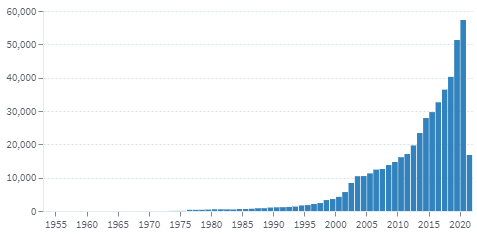
\includegraphics[width=.8\textwidth]{img/patentes/2a.png}
    \end{figure}

    \item Buscar patentes sobre “Fuzzy logic”. Indicar cuántas tiene “Microsoft” sobre esta temática.

    96.435 patentes. 4.696 + 2.141 del conglomerado de empresas de Microsoft.

    \begin{figure}[H]
        \centering
        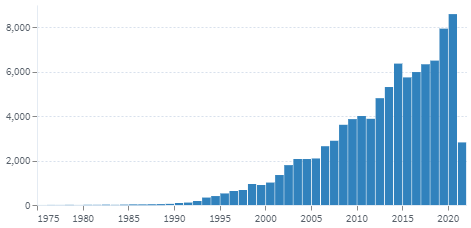
\includegraphics[width=.8\textwidth]{img/patentes/2b.png}
    \end{figure}

    \item Buscar patentes sobre “SVM” (Support Vector Machine). Indicar cuántas tiene “Microsoft” sobre esta temática.
    
    504.121 patentes. 6.829 + 5.415 del conglomerado de empresas de Microsoft.

    \begin{figure}[H]
        \centering
        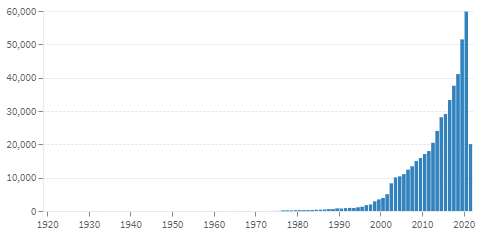
\includegraphics[width=.8\textwidth]{img/patentes/2c.png}
    \end{figure}
\end{itemize}

\subsection{}

Búsqueda de una patente y relación con patentes similares. Por ejemplo con Google Patents o Espacenet.

Buscar la patente WO2020033205A1. Indicar: 
\begin{itemize}
    \item \textbf{Los Inventores}: Stephen Alan Mckinley, David Gealy y Pieter Abbeel.
    \item \textbf{Institución o persona que realiza la solicitud}: Universidad de California.
    \item \textbf{Fecha de la solicitud}: 2019-07-31.
    \item \textbf{Fecha de la publicación}: 2020-02-13.
    \item \textbf{Códigos de Clasificación (CPC)}:
    \begin{itemize}
        \item B25J18/00 (US) 
        \item B25J9/0087 (EP)
        \item B25J9/102 (EP)
        \item B25J9/126 (EP,US)
        \item F16H48/38 (US) 
        \item B25J19/06 (US)
        \item F16H2048/387 (US)
    \end{itemize}
\end{itemize}


% Patentes
% 1) Quizás desarrollar un poco
% 2) Solo el número y (opcional) una gráfica
% 3) Solo las preguntas

% https://worldwide.espacenet.com/patent/search/family/069228268/publication/WO2020033205A1?q=WO2020033205A1